\section{Руководство пользователя}

Требуется убедиться, что серверная часть системы настроена. Для
начала работы необходимо запустить приложение на заранее известном ip адресе и порту. 

После запуска приложения пользователь получит доступ к интерактивной документации.
Чтобы получить доступ к интерактивной документации системы,
введите в адресной строке браузера URL /swagger. Например, если адрес
сервера – http://localhost:8080, то введите http://localhost:8080/swagger.
Нажмите клавишу Enter или выполните запрос, чтобы перейти на страницу с
интерактивной документацией.

В интерактивной документации показано описание
API-интерфейсов, которые могут использоваться для взаимодействия с
системой. Это набор методов, которые клиентские приложения могут
вызывать для выполнения различных операций в системе.

Описание API-интерфейсов включает информацию о доступных
методах, параметрах, возвращаемых значениях и кодах состояния HTTP.

На рисунках 5.1, 5.2, 5.3, 5.4, 5.5 показана интерактивная документация системы управления авторизацией, 
пользователями, категориями лотов, лотами, ставками соответсвенно.
\begin{figure}[h]
\centering
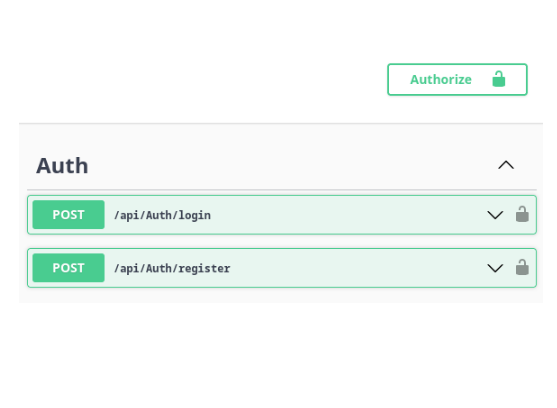
\includegraphics[scale=0.3]{511.png}
\caption{Интерактивная документация системы авторизации}
\end{figure}

% На рисунке 5.2 показана интерактивная документация системы управления пользователями.
\begin{figure}[h]
\centering
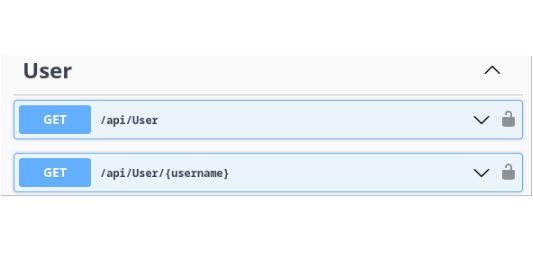
\includegraphics[scale=0.3]{522.png}
\caption{Интерактивная документация системы управления пользователями}
\end{figure}

% \newpage
% На рисунке 5.3 показана интерактивная документация системы управления категориями лотов.
\begin{figure}[h]
\centering
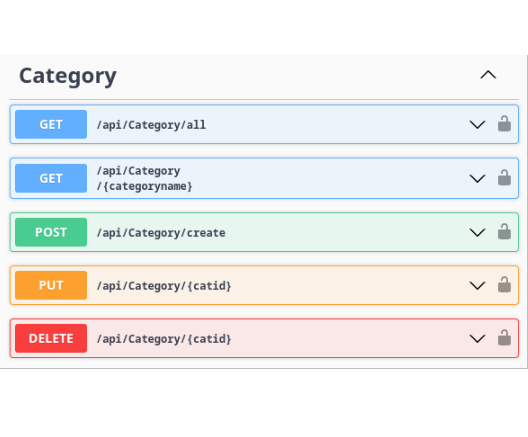
\includegraphics[scale=0.3]{533.png}
\caption{Интерактивная документация системы управления категориями лотов}
\end{figure}

% На рисунке 5.4 показана интерактивная документация системы управления лотами.
\begin{figure}[h]
\centering
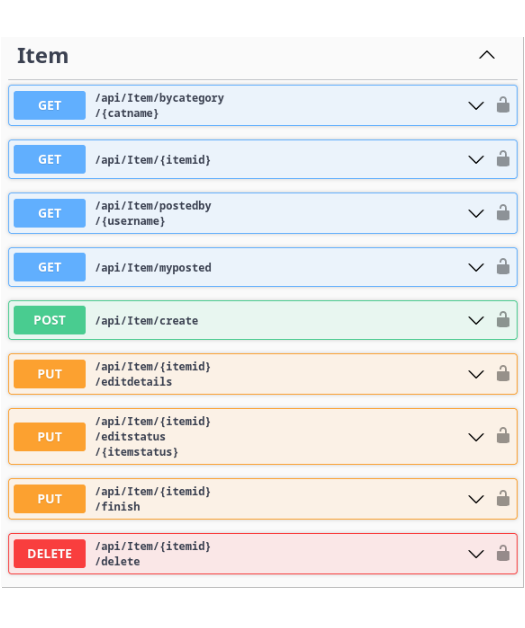
\includegraphics[scale=0.3]{544.png}
\caption{Интерактивная документация системы управления лотами}
\end{figure}

% На рисунке 5.5 показана интерактивная документация системы управления ставками.
\begin{figure}[h]
\centering
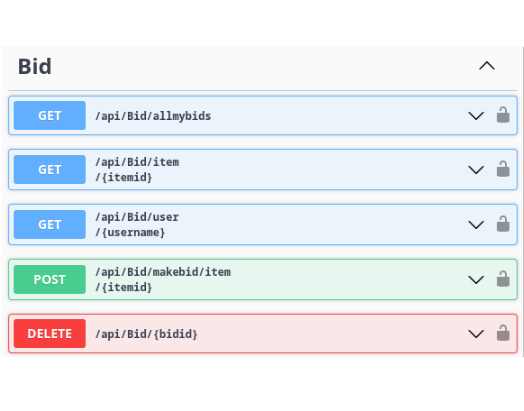
\includegraphics[scale=0.3]{555.png}
\caption{Интерактивная документация системы управления ставками}
\end{figure}